%
% chapter.tex -- Kapitel über Frames
%
% (c) 2019 Prof Dr Andreas Müller
%
\chapter{Frames
\label{chapter:frames}}
\lhead{Frames}
Analyse von Vektoren mit einer orthonormierten Basis führt auf eindeutige
Darstellungen. 
Ausserdem sind die Vektoren, die für Analyse und Synthese verwendet
werden, im Wesentlichen gleich.
Die Analyse erfolgt mit Hilfe einfacher Skalarprodukte mit den Basisvektoren.
Die zugehörige Transformationsmatrix ist orthogonal, so dass die
Matrix der Rücktransformation durch Transponieren gefunden werden kann.
Eine orthonormierte Basis ist daher sehr starr und oft gibt es für ein
Problem keine angemessene orthonormierte Basis.

In vielen Anwendungen muss daher der Begriff der Basis etwas aufgeweicht
werden:
\begin{enumerate}
\item
Es muss zugelassen werden, dass mehr Vektoren für die Analyse verwendet
werden, als strikt notwendig wäre.
Die Menge der Analyse-Vektoren ist daher nicht mehr eine Basis, man
verzichtet darauf, dass die Analyse-Vektoren {\em linear unabhängig} sein
müssen.
Man muss aber immer noch fordern, dass Vektoren nicht zu stark gestaucht
werden, damit Umkehrbarkeit der Transformation stetig möglich ist.
Auf diesem Weg gelangt man zum Begriff des {\em Frames}.
\item
Wenn die Vektoren nicht mehr linear unabhängig sind, ist es erst
recht nicht mehr möglich, dass sie orthonormiert sind.
Es muss daher auch zugelassen werden, dass einzelne Skalarprodukte 
$\langle v_i,v_j\rangle\ne 0$ sind für $i\ne j$.
Dies bedeutet aber dass die Transformationsmatrix nicht mehr so einfach
invertiert werden kann.
Analyse- und Synthese-Vektoren sind verschieden.
\end{enumerate}
In den folgenden Abschnitten wird erst in Abschnitt~\ref{section:frame}
der Begriff des motiviert und definiert.
In Abschnitt~\ref{section:dual} wird der Begriff des dualen Frames
eingeführt, die für die Synthese benötigt wird.
Die numerische Bestimmung des dualen Frames wird in
Abschnitt~\ref{section:ginv}.

%
% frame.tex
%
% (c) 2019 Prof Dr Andreas Müller, Hochschule Rapperswil
%

%
% Definition Frame
%
\begin{frame}
\frametitle{Frame}
\begin{definition}
Eine Menge von Vektoren $a_j$ heisst {\em Frame}, wenn
es Zahlen $B\ge A>0$ gibt mit
\[
A \|x\|^2
\le
\sum_{j} |\langle x,a_j\rangle|^2
\le
B \|x\|^2
\]
\uncover<2->{%
Das Frame heisst {\em straff}, wenn $A=B$.
}
\end{definition}
\begin{columns}[T,totalwidth=\textwidth]
\begin{column}{0.48\linewidth}
\uncover<3->{%
\begin{block}{Orthonormalbasis}
Falls $\mathcal{B}$ eine orthonormierte Basis,
dann ist $\mathcal{B}$ ein straffes Frame mit
$A=B=1$.
\end{block}
}
\end{column}
\uncover<4->{%
\begin{column}{0.48\linewidth}
\begin{block}{Mehrere Orthonormalbasen}
Falls $\mathcal{B}_i$ ein o.n.~Basis ist $1\le i\le n$,
dann ist
\[
\mathcal{B}
=
\bigcup_i \mathcal{B}_i
\]
ein straffes Frame mit $A=B=n$.
\end{block}
}
\end{column}
\end{columns}

\end{frame}

%
%
%
\begin{frame}
\frametitle{Dreiecksframe}
\centering
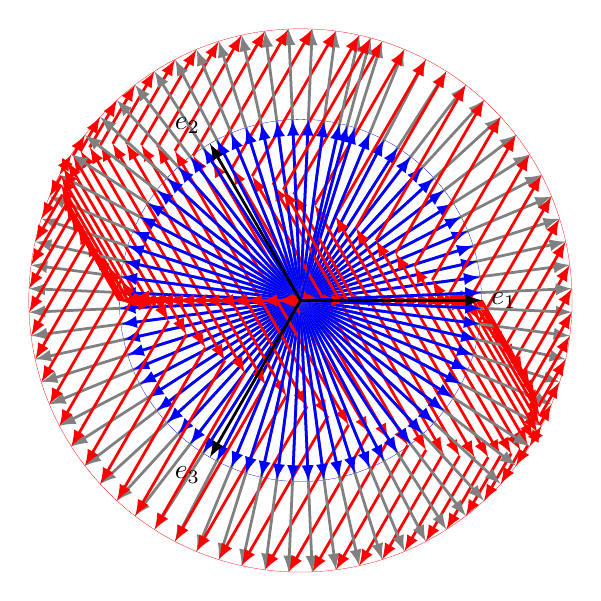
\begin{tikzpicture}[>=latex,scale=2.3]

\draw[color=red,line width=0.1pt] (0,0) circle[radius=1.5];
\draw[color=blue,line width=0.1pt] (0,0) circle[radius=1.0];

\ifthenelse{\boolean{presentation}}{
\foreach \A in {1,...,72}{
	\pgfmathparse{2.5+\A*5}
	\xdef\a{\pgfmathresult}

	\only<\A>{
	\draw[->,color=gray,line width=1pt] (0,0)--({1.5*cos(\a)},{1.5*sin(\a)});
	\draw[->,color=blue,line width=1pt] (0,0)--({cos(\a)},{sin(\a)});
	\pgfmathparse{cos(\a)}
	\xdef\x{\pgfmathresult}
	\pgfmathparse{sin(\a)}
	\xdef\y{\pgfmathresult}
	\draw[->,color=red,line width=1pt]
		(0,0)--({\x},0);
	\pgfmathparse{(-0.5)*\x+\y*(sqrt(3)/2)}
	\xdef\B{\pgfmathresult}
	\pgfmathparse{(-0.5)*\x+\y*(-sqrt(3)/2)}
	\xdef\C{\pgfmathresult}
	\draw[->,color=red,line width=1pt]
		({\x},0)--({\x-0.5*\B},{0+\B*sqrt(3)/2});
	\draw[->,color=red,line width=1pt]
		({\x-0.5*\B},{0+\B*sqrt(3)/2})
		--({\x-0.5*\B-0.5*\C},{0+\B*sqrt(3)/2-\C*sqrt(3)/2});
	}
}
}{
	\xdef\a{75}

	\draw[->,color=gray,line width=1pt] (0,0)--({1.5*cos(\a)},{1.5*sin(\a)});
	\draw[->,color=blue,line width=1pt] (0,0)--({cos(\a)},{sin(\a)});
	\pgfmathparse{cos(\a)}
	\xdef\x{\pgfmathresult}
	\pgfmathparse{sin(\a)}
	\xdef\y{\pgfmathresult}
	\draw[->,color=red,line width=1pt]
		(0,0)--({\x},0);
	\pgfmathparse{(-0.5)*\x+\y*(sqrt(3)/2)}
	\xdef\B{\pgfmathresult}
	\pgfmathparse{(-0.5)*\x+\y*(-sqrt(3)/2)}
	\xdef\C{\pgfmathresult}
	\draw[->,color=red,line width=1pt]
		({\x},0)--({\x-0.5*\B},{0+\B*sqrt(3)/2});
	\draw[->,color=red,line width=1pt]
		({\x-0.5*\B},{0+\B*sqrt(3)/2})
		--({\x-0.5*\B-0.5*\C},{0+\B*sqrt(3)/2-\C*sqrt(3)/2});
}

\draw[->,line width=1pt] (0,0)--(1,0);
\draw[->,line width=1pt] (0,0)--(-0.5,{sqrt(3)/2});
\draw[->,line width=1pt] (0,0)--(-0.5,{-sqrt(3)/2});
\node at (1,0) [right] {$e_1$};
\node at (-0.5,{sqrt(3)/2}) [above left] {$e_2$};
\node at (-0.5,{-sqrt(3)/2}) [below left] {$e_3$};
\end{tikzpicture}
\end{frame}

%
%
%
\begin{frame}
\frametitle{Straffe Frames}
Gram-Operator:
\[
Gx = \sum_{j} \langle x,a_j\rangle a_j
\]
\end{frame}

%
% dual.tex -- duale frames
%
% (c) 2019 Prof Dr Andreas Müller, Hochschule Rapperswil
%
\section{Das duale Frame\label{section:dual}}
\rhead{Das duale Frame}
In diesem Abschnitt gehen wird davon aus, dass $\mathcal{B}$ ein
Frame in $\mathbb{R}^n$ ist mit Framekonstanten $A$ und $B$.
Die Transformation $\mathcal{T}$, die zu diesem Frame gehört, liefert 
zu einem Vektor $v$ die Analysekoeffizienten $\hat{v} = \mathcal{T}v$.
Die Konstruktion eines Filters auf der Basis einer solchen Analyse verlangt
jedoch auch, dass die Abbildung $\mathcal{T}$ umgekehrt werden kann.
Von vornherein ist aber nicht klar, ob die Abbildung überhaupt umkehrbar ist,
denn es wurde ja nicht verlangt, dass die Framevektoren linear unabhängig
sind.
Im besten Fall kann man also Linksinverse von $\mathcal{T}$ erwarten.
\index{Linksinverse}
Eine solche ordnet jedem Koeffizienten $\hat{v}_k$ einen Vektor $v_k'$
zu, das sogenannte duale Frame, welches in diesem Abschnitt konstruiert
werden soll.

Wir betrachten in diesem Abschnitt immer ein Frame $\mathcal{B}$
mit Framevektoren $b_k$ und Framekonstanten $A$ und $B$.
Der Frameoperator $\mathcal{T}$ ordnet dem Vektor $v\in V$ den Vektor
mit Koordinaten $\hat{v}_k$ zu.

\subsection{Der Gram-Operator}
Das Frame $\mathcal{B}$ mit den Framekonstanten $A$ und $B$ erfüllt
\[
A\|v\|^2 \le \sum_{k=1}^m |\langle v,b_k\rangle|^2 \le B\|v\|^2
\qquad\forall v\in \mathbb R^n.
\]
Die Quadratsumme in der Mitte ist genau die Norm des Vektors
$\hat{v}$ in $\mathbb R^m$.
Unterscheiden wir für den Moment die verschiedenen Skalarprodukte
und Normen dadurch, dass wir die Vektorräume als Indizes hinzufügen,
können wir die Frameungleichung schreiben als
\[
A \| v\|_{\mathbb R^n}^2
\le
\| Tv\|_{\mathbb R^m}^2
\le
B \| v\|_{\mathbb R^n}^2.
\]
Die Norm von $Tv$ in $\mathbb R^m$ ist
\[
\| Tv\|_{\mathbb R^m}^2
=
\langle Tv,Tv\rangle_{\mathbb R^m}
=
(Tv)^tTv
=
v^t(T^tT)v
=
\langle T^tTv,v\rangle_{\mathbb R^n}.
\]
Man beachte, dass $T^tT$ eine symmetrische $n\times n$-Matrix ist,
die codiert, wie stark die einzelnen Vektoren $v\in\mathbb R^n$ durch
den Frameoperator $\mathcal{T}$ verzerrt werden.
Dies rechtfertigt eine eigene Definition.

\begin{definition}
\label{definition:gram-operator}
\index{Gram-Operator}
Ist $T$ die Matrix des Frameoperators $\mathcal{T}$ eines Frames
$\mathcal{B}$, dann heisst $G=T^tT$ der {\em Gramoperator} des Frames
$\mathcal{B}$.
\end{definition}

Die Framebedingung lässt sich mit dem Gram-Operator $T^tT$ als
\begin{equation}
A \|v\|^2
\le
\langle T^t T v,v\rangle
\le
B \|v\|^2
\label{framebedingung:ttt}
\end{equation}
schreiben.
Man kann daraus schliessen, dass der Gram-Operator $T^tT$ regulär ist.

Die symmetrische Matrix $T^tT$ kann durch Wahl einer geeigneten Basis
in $\mathbb R^n$ diagonalisiert werden.
Die Eigenvektoren können sogar orthonormiert gewählt werden.
Seien daher $u_1,\dots,u_n$ orthonormierte Eigenvektoren von $T^tT$
mit Eigenwerten $\lambda_1\le\dots\le\lambda_n$.
Die Framebedingung~\eqref{framebedingung:ttt}
für den Vektore $v=u_k$ sagt dann
\[
A \| u_k\|^2
=
A
\le
\langle T^tTu_k,u_k\rangle
=
\lambda_k\langle u_k,u_k\rangle
=
\lambda_k
=
B \| u_k\|^2
=
B.
\]
Die Eigenwerte von $T^tT$ sind also alle zwischen $A$ und $B$.
Man kann sogar noch mehr sagen:

\begin{satz}
Sei $\mathcal{B}\subset\mathbb R^n$ eine Menge von Vektoren derart,
dass die zugehörige Matrix $T^tT$ regulär ist.
Seien weiter $\lambda_1\le\dots\le \lambda_n$ die Eigenwerte
(mit Vielfachheiten) von $T^tT$.
Dann ist $\mathcal{B}$ ein Frame mit Framekonstanten
$A=\lambda_1$ und $B=\lambda_n$.
\end{satz}

\begin{beispiel}
Im Beispiel von Abschnitt~\ref{subsection:hexagon} ist die Matrix $T$
gegeben in \eqref{beispielTmatrix}.
Der zugehörige Gram-Operator ist
\[
T^tT
=
\begin{pmatrix}
1& -\frac12        &-\frac12          \\[2pt]
0& \frac{\sqrt{3}}2& -\frac{\sqrt{3}}2
\end{pmatrix}
\begin{pmatrix}
1&0\\
-\frac12&\frac{\sqrt{3}}2\\[2pt]
-\frac12&-\frac{\sqrt{3}}2
\end{pmatrix}
=
\begin{pmatrix}
1+\frac14+\frac14 & 0-\frac{\sqrt{3}}4+\frac{\sqrt{3}}4\\[2pt]
0-\frac{\sqrt{3}}4+\frac{\sqrt{3}}4&0+\frac{3}{4}+\frac{3}{4}
\end{pmatrix}
=
\begin{pmatrix}
\frac32&0\\
0&\frac32
\end{pmatrix}
=
\frac{3}{2}E
\]
Da die Matrix $T^tT$ bereits diagonal ist, können die Eigenwerte
$\lambda_1=\lambda_2=\frac32$ direkt abgelesen werden.
\end{beispiel}

Das Frame des Beispiels ist straff und der Gram-Operator ist ein
Vielfaches der Einheitsmatrix.
Dies ist kein Zufall, wie das folgende Korollar zeigt.

\begin{korollar}
Das Frame $\mathcal{B}$ ist genau dann straff, wenn der zugehörige
Gram-Operator $T^tT$ ein Vielfaches der Einheitsmatrix ist.
\end{korollar}

\begin{figure}
\centering
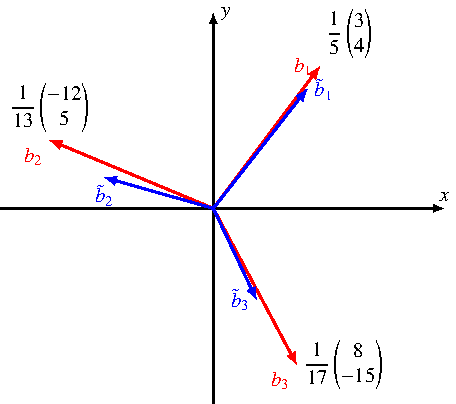
\includegraphics{chapters/1-geometrie/images/beispiel2.pdf}
\caption{Beispiel eines nicht straffen Frames mit rationalen Framevektoren
$b_k$ (rot).
Die Vektoren $\tilde{b}_k$ des dualen Frames
(siehe Definition~\ref{definition:dualesframe}) sind blau eingezeichnet.
\label{frame:beispiel2}}
\end{figure}

\begin{beispiel}
Die Vektoren
\[
\mathcal{B} 
=
\biggl\{
\frac15
\begin{pmatrix} 3\\4\end{pmatrix},
\frac1{13}
\begin{pmatrix} -12\\5\end{pmatrix},
\frac1{17}
\begin{pmatrix} 8\\-15\end{pmatrix}
\biggr\}
\subset \mathbb R^2
\]
erzeugen den ganzen Raum $\mathbb R^2$, sie bilden daher ein
Frame (Abbildung~\ref{frame:beispiel2}).
Wir berechnen den Frame-Operator, den Gram-Operator und seine Eigenwerte,
um die Framekonstanten zu ermiteln.

Der Frame-Operator ist die Matrix
\[
T
=
\begin{pmatrix}
 \frac{ 3}{ 5}& \frac{ 4}{ 5}\\[2pt]
-\frac{12}{13}& \frac{ 5}{13}\\[2pt]
 \frac{ 8}{17}&-\frac{15}{17}
\end{pmatrix}.
\]
Der Gram-Operator wird daher
\[
G=T^tT
=
\begin{pmatrix}
 \frac{ 3}{ 5}&-\frac{12}{13}&  \frac{ 8}{17}\\[2pt]
 \frac{ 4}{ 5}& \frac{ 5}{13}& -\frac{15}{17}
\end{pmatrix}
\begin{pmatrix}
 \frac{ 3}{ 5}& \frac{ 4}{ 5}\\[2pt]
-\frac{12}{13}& \frac{ 5}{13}\\[2pt]
 \frac{ 8}{17}&-\frac{15}{17}
\end{pmatrix}
=
\frac{1}{1221025}
\begin{pmatrix}
1750369&  286808 \\
 286808& 1676106
\end{pmatrix}
\]
Die Eigenwerte dieser $2\times 2$-Matrix können als Nullstellen des
charakteristischen Polynoms mit der Lösungsformel für quadratische
Gleichungen berechnet werden.
Man findet zum Beispiel mit Hilfe eines Computer-Algebra-Systems
\[
\lambda_{\pm}
=
\frac{52715\pm 41\sqrt{47105}}{37570}
\quad\Rightarrow\quad
\left\{
\begin{aligned}
A&=
1.166262672548251
\\
B&=
1.639965701154171.
\end{aligned}
\right.
\]
Da die beiden Konstanten nicht übereinstimmen, ist dieses Frame
nicht straff.
\end{beispiel}

\begin{proof}[Beweis des Korollars]
Ein straffes Frame hat $A=B$, was gleichbedeutend damit ist, dass
die Eigenwerte des Frameoperators $T^tT$ mit 
$A=B=\lambda_1=\dots=\lambda_n$ übereinstimmen.
Dies wiederum ist gleichbedeutend damit, dass alle Vektoren Eigenvektoren
zum gleichen Eigenwert sind und $T^tT=AE=BE$.
\end{proof}

\subsection{Die inverse Abbildung des Frameoperators}
Für ein straffes Frame gilt $T^tT  = AE$.
Bis auf den Faktor $A$ ist daher $T^t$ bereits eine Linksinverse von $T$.
Genauer, mit
\[
S=\frac1{A} T^t
\qquad\text{folgt}\qquad
ST
=
\frac1{A} T^tT
=
\frac1{A} AE
=
E.
\]
Eine Linksinverse von $\mathcal{T}$ ist also für ein straffes Frame
leicht zu finden.

Für ein beliebiges Frame lässt sich ebenfalls eine Linksinverse angeben.
Mit $G=T^tT$ ist
\[
v
=
\underbrace{G^{-1}T^t}_{\displaystyle=S}Tv
=
STv,
\]
die Matrix $S=G^{-1}T^t$ ist also die gesuchte Linksinverse von $T$.

\subsection{Das duale Frame}
\index{duales Frame}
\index{Frame!duales}
Um den Frameoperator umzukehren, muss man $G^{-1}T^t$ berechnen
können.
Auf einen Vektor $\hat{v} = (\hat{v}_k)_{1\le k\le m} = Tv$ angewendet
bedeutet dies, dass man $G^{-1}$ auf
\[
T^t \hat{v} = \sum_{k=1}^m \hat{v}_k  b_k
\]
anwenden muss, dabei wurde verwendet, dass $T^t$ als Spalten die
Vektoren $b_k$ enthält.
Anwendung von $G^{-1}$ liefert
\[
v
=
G^{-1} T^t \hat{v}
=
\sum_{k=1}^m \hat{v}_k G^{-1}b_k.
\]
Den Vektor $v$ erhält man also als Linearkombination der Vektoren
\[
\tilde{\mathcal{B}}
=
\{ G^{-1}b_1,\dots,G^{-1}b_n\}
=
\{ \tilde{b}_k = G^{-1}b_k\,|\, 1\le k\le m\}.
\]

\begin{definition}
\label{definition:dualesframe}
Ist $\mathcal{B}=\{b_1,\dots,b_m\}$, dann heisst
$\tilde{\mathcal{B}} = \{\tilde{b}_1,\dots,\tilde{b}_m\}$ 
mit
$\tilde{b}_k=G^{-1} b_k$
das zu $\mathcal{B}$ duale Frame.
\end{definition}

\begin{beispiel}
Das duale Frame zum Beispiel zu Abbildung~\ref{frame:beispiel2} kann
ebenfalls mit Hilfe eines Computer-Algebra-Systems berechnet werden aus
der bereits früher berechneten Matrix bestimmt werden.
Aus 
\[
G^{-1}T^t
=
\begin{pmatrix}
\frac{4259}{8053}
	&-\frac{718432}{1167685}
		&\frac{284716}{1167685}\\[2pt]
\frac{5422}{8053}
	&\frac{408473}{2335370}
		&-\frac{1203549}{2335370}
\end{pmatrix}
=
\begin{pmatrix}
0.52887&-0.61526&\phantom{-} 0.24383\\
0.67329&\phantom{-} 0.17490&-0.51536
\end{pmatrix}
\]
findet man das duale Frame
\[
\tilde{\mathcal{B}}
=
\left\{
\begin{pmatrix}
\frac{4259}{8053}\\[2pt]
\frac{5422}{8053}
\end{pmatrix},
\begin{pmatrix}
-\frac{718432}{1167685}\\[2pt]
\frac{408473}{2335370}
\end{pmatrix},
\begin{pmatrix}
\frac{284716}{1167685}\\[2pt]
-\frac{1203549}{2335370}
\end{pmatrix}
\right\}
=
\left\{
\begin{pmatrix} 0.52887\\ 0.67329 \end{pmatrix},
\begin{pmatrix}-0.61526\\ \phantom{-}0.17490 \end{pmatrix},
\begin{pmatrix}\phantom{-}0.24383\\ -0.51536 \end{pmatrix}
\right\}.
\]
Die Vektoren des dualen Frames sind in Abbildung~\ref{frame:beispiel2}
blau eingezeichnet.
\end{beispiel}

\begin{korollar}
Ist $\mathcal{B}=\{b_1,\dots,b_m\}$ ein straffes Frame mit Framekonstanten
$A=B$, dann ist
\[
\tilde{\mathcal{B}}
=
\biggl\{\tilde{b}_k = \frac1Ab_k\,\bigg|\,1\le k\le m\biggr\}
\]
das dazu duale Frame.
\end{korollar}

\begin{proof}[Beweis]
Für ein straffes Frame ist $T^tT=AE$, also ist $G^{-1}=\frac1A E$.
Die Vektoren des dualen Frames sind daher
$\tilde{b}_k = \frac1AEb_k=\frac1Ab_k$.
\end{proof}

Die Linksinverse $S$ von $\mathcal{T}$ kann mit Hilfe des dualen Frames
sehr leicht formuliert werden.

\begin{satz}
Ist $\mathcal{B}$ ein Frame und $\tilde{\mathcal{B}}$ das dazu duale
Frame und ist $\hat{v} = Tv$, dann ist die Linksinverse $S$ von $T$
gegeben durch
\[
v
=
S\hat{v}
=
\sum_{k=1}^m \hat{v}_k \tilde{b}_k.
\]
Linearkombination der Vektoren des dualen Frames mit den Analysekoeffizienten
$\hat{v}_k$ liefert also das ursprüngliche Signal zurück.
\end{satz}

\begin{beispiel}
\label{beispiel3}
In diesem Beispiel betrachten wir das Frame bestehend aus den
Signalen, die auf einem von maximal elf Samples konstant sind
und sonst verschwinden.
Das Signal $b_k$ verschwindet für Samples $i>k$ und $i<k-10$
und ist so normiert, dass $\|b_k\|=1$.
Die zugehörigen dualen Signale können direkt berechnet werden,
zwei Beispiele sind in den Abbildungen \ref{b3-01} und \ref{b3-05}
dargestellt.
\def\beispieldrei#1#2{
\begin{figure}
\centering
\includegraphics{chapters/1-geometrie/images/b3-#1.pdf}
\caption{Signal $b_{#2}$ aus dem Beispiel von Seite~\pageref{beispiel3}
und zugehöriges duales Signal $\tilde{b}_{#2}$.
\label{b3-#1}}
\end{figure}
}
\beispieldrei{01}{1}
%\beispieldrei{02}{3}
%\beispieldrei{03}{6}
%\beispieldrei{04}{10}
\beispieldrei{05}{20}
%\beispieldrei{06}{30}
%\beispieldrei{07}{40}
%\beispieldrei{08}{50}
%\beispieldrei{09}{60}
%\beispieldrei{10}{70}
\end{beispiel}

In der Definition~\ref{definition:dualesframe} wird das duale Frame
definiert ohne zu rechtfertigen, dass die Vektoren $\tilde{b}_k$ 
tatsächlich ein Frame bilden.
Wegen $b_k=G\tilde{b}_k$ ist aber klar, dass die Vektoren $\tilde{b}_k$
den ganzen Vektorraum $\mathbb R^n$ erzeugen.
Insbesondere bilden sie ein Frame.
Damit sind jedoch die Framekonstanten noch nicht bestimmt.
Dies wird im folgenden Satz nachgeholt.

\begin{satz}
Ist $\mathcal{B}=\{b_1,\dots,b_m\}$ ein Frame mit Framekonstanten
$A$ und $B$, dann hat das duale Frame die Framekonstanten $1/B$ und $1/A$.
\end{satz}

\begin{proof}[Beweis]
Um die Framekonstanten des dualen Frames zu bestimmen,
müssen der Frameoperator $\tilde{T}$ und Gram-Operator $\tilde{G}$
des dualen Frames bestimmt werden.
Das duale Frame besteht aus den Spaltenvektoren von $S=G^{-1}T^t$,
also ist der Frameoperator $\tilde{T}=S^t$ und damit ist der Gram-Operator
\[
\tilde{G}
=
\tilde{T}^t\tilde{T}
=
(S^t)^tS^t
=
SS^t
=
G^{-1}T^tTG^{-1}
=
G^{-1}.
\]
Der Gram-Operator des dualen Frames ist daher die Inverse des
Gram-Operators des ursprünglichen Frames.
Sind $A=\lambda_1\le \dots\le \lambda_n=B$ die Eigenwerte  von $G$,
dann sind
$1/B\le \lambda_n^{-1} \le \dots \le \lambda_1^{-1}\le 1/A$ 
die Eigenwerte von $\tilde{G}=G^{-1}$.
Daraus folgen die behaupteten Framekonstanten.
\end{proof}

%
% Allgemeine Frames
%
\subsection{Allgemeine Frames}
Die Wahl der Indexmenge $K$ in der Definition~\ref{definition:frame}
war einigermassen willkürlich.
Schon bei der Fouriertransformation ist eine solche diskrete Menge
für die Indizierung der Vergleichsfunktionen nicht mehr ausreichend.
Dort werden nämlich die Funktion $e^{i\omega t}$ mit $\omega\in\mathbb R$
verwendet.
Auch die geplante Anwendung auf Wavelets ist davon betroffen.
Dort wollen wir mit Funktionen $\psi_{a,b}$ vergleichen, die 
skalierte und verschobene Versionen eines Mutterwavelets $\psi$ sind,
mit Skalierungsfaktor $a\in\mathbb R^*$ und die Translationsdistanz
$b\in \mathbb R$.
\index{Skalierungsfaktor}%
\index{Translationsdistanz}%

Lässt man eine beliebige Indexmenge zu, ist die Definition der
Transformation $T$
\[
k
\mapsto
(Tv)(k) = \langle v,e_k\rangle
\]
als komplexwertige Funktion auf $K$ immer noch sinnvoll.
Für eine überabzählbare Indexmenge $K$ ist die Summe 
\[
\sum_{k\in K} |\langle v,e_k\rangle|^2,
\]
die in der Definition eines Frames auftritt, schlicht sinnlos.
Wir stehen hier also vor einem ähnlichen Problem wie bei der Frage,
wie man aus dem Raum der Signale auf $\mathbb R$ einen Hilbertraum machen kann.
Diese Frage wird in Kapitel~\ref{chapter:fourier} im Detail beantwortet.

Nehmen wir für den Moment an, dass es gelungen ist, eine Hilbertraum $H$
von Funktionen auf $K$ zu konstruieren.
Die Frameungleichung kann dann mit Hilfe der Norm von $H$ formuliert
werden, sie lautet
\[
A\|v\|^2 \le \|Tv\|^2 \le B\|v\|^2.
\]
Die Norm in der Mitte ist als Norm in $H$ zu lesen.
Diese Ungleichungen sagen immer noch aus, dass kein Vektor $v\in V$ bei
der Transformation $T$ ``unsichtbar'' wird.
Wäre nämlich $Tv=0$ in $H$, dann wäre auch $\|Tv\|=0$ und damit
$\|v\|=0$.
Die Frameungleichung stellt also sicher, dass die Abbildung $T$ 
injektiv und damit potentiell invertierbar ist.

Es ist aber keinesfalls garantiert, dass das Bild der Transformation $T$
den ganzen Hilbertraum $H$ abdeckt, ganz im Gegenteil.
Schon im Beispiel in Abschnitt~\ref{subsection:hexagon} wurde gezeigt,
dass die mit Hilfe eines Frames gefundenen Koeffizienten redundant sind.
Alle Vektoren der Menge
\[
\left\{
\left.
\begin{pmatrix}\hat{v}_1\\\hat{v}_2\\\hat{v}_3\end{pmatrix}
+\alpha\begin{pmatrix}1\\1\\1\end{pmatrix}
\,
\right|\,
\alpha \in\mathbb R
\right\}
\]
beschreiben den gleichen Punkt in der Ebene, aber nur einer davon 
wird von der Transformation $T$ erreicht.
Dies entspricht natürlich genau dem, was man erwartet: der Bildraum
der Ebene $\mathbb R^2$ unter der Abbildung $T$ ist ein zweidimensionaler
Teilraum des $\mathbb R^3$.

Die Abbildung $T$ wird daher im Allgemeinen nicht invertierbar sein, aber
wir dürfen hoffen, dass es eine Formel gibt, mit der man aus $Tv$ den 
Vektor $v$ rekonstruieren kann.
Im Falle des Beispiels war dies die Formel
\[
v = \frac23 \sum_{k=1}^3 \langle v,e_k\rangle \, e_k.
\]
Für ein beliebiges Frame ist so eine Formel natürlich wieder wegen
der Summe nicht sinnvoll.
Doch in Kapitel~\ref{chapter:fourier} werden wir sehen, dass sie sich
oft durch eine Integralformel ersetzen lässt.
Die Konstruktion eines solchen vektorwertigen Integrals ist allerdings
etwas subtil, wird kehren zu dieser Problematik im Kapitel~\ref{chapter:cwt}
zurück.



%
% ginv.tex -- Invertierung des Gram-Operators
%
% (c) 2019 Prof Dr Andreas Müller, Hochschule Rapperswil
%
\section{Invertierung des Gram-Operators\label{section:ginv}}
\rhead{Invertierung des Gram-Operators}
\index{Invertierung des Gram-Operators}
Die Bestimmung des dualen Frame setzt voraus, dass der Gram-Operator
$G$ invertiert werden kann.
Eine linksinverse Transformation zum Frameoperator $M$ ist dann durch
$S=G^{-1}T^t$ gegeben.

Da $G$ eine positiv definite symmetrische Matrix mit Spektrum im
Intervall $[A,B]$ ist, ist die Matrix in der Eigenbasis sehr einfach
zu invertieren.
Die Eigenvektoren zu finden ist jedoch eine noch deutlich aufwendigere
Aufgabe, als die Matrix $G$ zu invertieren.
Ausserdem gibt es kein Interesse, in der Eigenbasis zu arbeiten, alle
Operationen sollen in der durch das Frame vorgegebenen Basis durchgeführt
werden.

Eine Linksinverse von $T$ zu finden ist gleichbedeutend damit,
die dualen Framevektoren $b_i' = Sb_i = G^{-1}Tb_i$ zu bestimmen.
Ziel dieses Abschnitts ist daher, einen spezialisierten numerischen
Algorithmus zu finden, der jeden der Vektoren $b_i'$ finden kann.

In der Eigenbasis von $G$ läuft die Invertierung von $G$ auf
das Invertieren der Eigenwerte hinaus.
Wir suchen daher in \ref{subsection:reziprok} erst einen iterativen
Algorithmus, der $1/\lambda$ berechnen kann für $\lambda\in[A,B]$.
In \ref{subsection:ginv} verallgemeinern wir diesen Algorithmus
anschliessend auf die Bestimmung von $G^{-1}$ bzw.~$b_i'$.

\subsection{Iterative Berechnung eines reziproken Wertes
\label{subsection:reziprok}}
Zu einer beliebigen Zahl $y$ mit $A < y < B$ muss der reziproke Wert $1/y$
bestimmt werden.
Wir suchen nach einem iterativen Verfahren der Form $x_{n+1}=f(x_n)$,
welches für einen beliebigen Startwert $x_0$ gegen $y^{-1}$ konvergiert
aber die Division nicht verwendet (da die Bestimmung der inversen
Matrix ja vermieden werden soll).
Der Wert $y^{-1}$ muss also der einzige Fixpunkt der Funktion $f(x)$ sein:
$f(y^{-1})=y^{-1}$.

Die Funktion $f(x) = x + g(x)$ hat als einzigen Fixpunkt die Stelle $x=y^{-1}$
genau dann, wenn $g(x)$ als einzige Nullstelle die Stelle $x=y^{-1}$ hat.
Ausserdem muss die Funktion $g(x)$ berechenbar sein ausschliesslich mit
Addition und Multiplikation von Konstanten und der Variablen $x$, Division
darf nicht verwendet werden.
Die einfachste Funktion dieser Art ist eine lineare Funktion, zum 
Beispiel $g(x) = 1- xy$.

\begin{figure}
\centering
\begin{tabular}{cc}
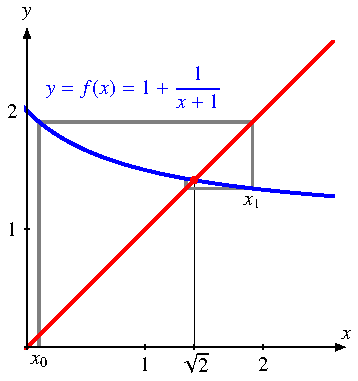
\includegraphics{chapters/1a-frames/images/ibkonv.pdf}&
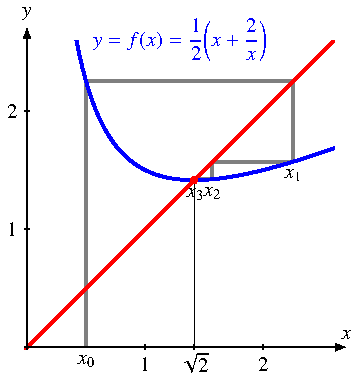
\includegraphics{chapters/1a-frames/images/itkonv.pdf}\\
(a)&(b)
\end{tabular}
\caption{Konvergenzeigenschaften eines Iterationsverfahrens der Form
$x_{n+1}=f(x_n)$.
Die Konstruktion des grauen Pfades ist im Text auf
Seite~\pageref{frame:grauerpfad} erklärt.
In beiden Fällen ist $\bar{x}=\sqrt{2}$ ein Fixpunkt der Funktion $f$.
Falls $|f'(\bar{x})| < 1$, konvergiert die Iterationsfolge linear, wie in (a)
erkennbar.
Für $f'(\bar{x})=0$ ist die Konvergenz besonders schnell (quadratische
Konvergenz), wie man in (b) sehen kann.
\label{frame:iterationsvergleich}}
\end{figure}

\begin{figure}
\centering
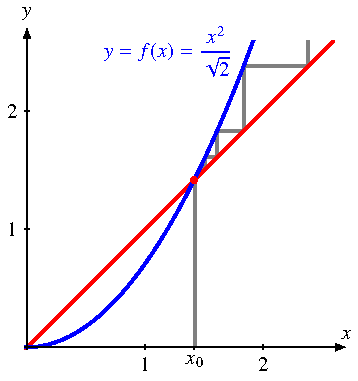
\includegraphics{chapters/1a-frames/images/div.pdf}
\caption{Konvergenzeigenschaften eines Iterationsverfahrens der Form
$x_{n+1}=f(x_n)$.
Für $|f'(\bar{x})|>1$ divergiert die Iterationsfolge (c).
\label{frame:divergenz}}
\end{figure}

Damit das Iterationsverfahren konvergiert, sind aber noch weitere
Bedingungen zu erfüllen (Abbildungen~\ref{frame:iterationsvergleich}
und \ref{frame:divergenz}).
Das Konvergenzverhalten kann wie folgt visualisiert werden.
Die Auswertung der Funktion $\color{blue}f(x_n)$ zeigen wir durch
eine Strecke von $(x_n,x_n)$ nach $\color{blue}(x_n,f(x_n))$ auf
dem blauen Graphen der Funktion $f$.
Die nächste Iteration startet mit $x_{n+1} = f(x_n)$, wir illustrieren
dies durch eine Strecke zum Punkt $\color{red}(f(x_n),f(x_n))$ auf der
Winkelhalbierenden des ersten Quadranten.
Auf diese Weise entsteht der graue Pfad in den Abbildungen.
\label{frame:grauerpfad}
Er führt jeweils vom blauen Graphen horizontal zur Winkelhalbierenden
und von dort vertikal wieder zum blauen Graphen.

Aus den Abbildungen kann man die folgende Bedingung für die Konvergenz
ablesen, die sich auch streng beweisen lässt.
Die Folge $x_{n+1} = f(x_n)$ konvergiert nur, wenn die Steigung
der Funktion $f(x)$ in der Nähe des Fixpunktes Betrag $<1$ hat, 
also $|f'(x)|<1$.
Für die eben konstruierte Funktion trifft dies im Allgemeinen nicht zu,
es ist nämlich
\[
f'(x) = 1 + g'(x) = 1 - y.
\]
Für $y>2$ wird nämlich $|f'(x)|'=|1-y| = y-1 >1$, so dass keine Konvergenz
mehr möglich ist.
Allerdings ist Konvergenz auch nicht für alle Werte von $y$ nötig, sondern
nur für Werte zwischen $A$ und $B$.
Das kann man mit Hilfe eines Skalierungsfaktors $c$ in der Iteration
\[
f(x) = x + c(1-yx)
\]
erreichen.
Die Ableitung wird damit
\[
f'(x) = 1-cy.
\]
$c$  muss also so gewählt werden, dass $|f'(x)|<1$ gilt für alle $y$
zwischen $A$ und $B$.
Dies bedeutet, dass
\begin{align*}
-1 &< 1-cy < 1 \\
-2 &< -cy < 0 \\
2 &> cy > 0 \\
\frac1c &> \frac{y}2.
\end{align*}
Diese Ungleichung muss für alle möglichen Werte für $y$ erfüllt sein,
also sowohl für $y=A$ also auch für $y=B$.
Man kann dies zum Beispiel dadurch erreichen, dass man
\[
\frac1c = \frac{A}2 + \frac{B}2
\qquad\Rightarrow\qquad
c = \frac{2}{A+B}
\]
setzt.

Damit haben wir jetzt ein Iterationsverfahren zur Berechnung des 
reziproken Wertes, welches wir im folgenden Satz zusammenfassen.

\begin{satz}
\label{satz:reziprok}
Ist $y$ eine reelle Zahl zwischen $A$ und $B$, $A\le y\le B$ dann
konvergiert die Folge
\[
x_{n+1} = x_n + \frac{2}{A+B}(1-yx_n), \quad x_0 = 0
\]
gegen den reziproken Wert $y^{-1}$ von $y$.
Die Differenz zwischen aufeinanderfolgenden Approximationen nimmt
in jedem Schritt um mindestens den Faktor $(B-A)/(B+A)<1$ ab.
\end{satz}

Die Fehler verhalten sich also wie eine geometrische Folge.
\index{geometrische Folge}%
Man nennt diese Art von Konvergenz, bei der der Fehler in jedem
Schritt um den gleichen Faktor kleiner wird auch {\em lineare Konvergenz},
\index{lineare Konvergenz}%
weil die Anzahl der korrekten Stellen in jedem Schritt um gleichen
Wert zunimmt.

\begin{proof}[Beweis]
Wir müssen uns nur noch mit der Aussage über die Konvergenz befassen.
Dazu berechnen wir die Differenz zweier aufeinanderfolgender
Approximationen 
\begin{equation}
\left.
\begin{aligned}
x_{n+1} &= x_n + \frac{2}{A+B}(1-yx_n) \\
x_n &= x_{n-1} + \frac{2}{A+B}(1-yx_{n-1}) 
\end{aligned}
\right\}
\quad\Rightarrow\quad
x_{n+1}-x_n
=
x_n - x_{n-1} -\frac{2y}{A+B}(x_n-x_{n-1})
=
\underbrace{
\biggl(1-\frac{2y}{A+B}\biggr)
}_{\displaystyle=\vartheta}
(x_n - x_{n-1}).
\end{equation}
Die Differenz nimmt also tatsächlich um den Faktor $\vartheta$ ab.
Wir schätzen diesen Faktor ab
\[
\vartheta
=
1-\frac{2y}{A+B} = \frac{A+B-2y}{A+B}
\qquad
\Rightarrow
\qquad
|\vartheta|
<
\biggl|\frac{A+B-2B}{A+B}\biggr|
=
\biggl|\frac{A-B}{A+B}\biggr|
=
\frac{B-A}{B+A}.
\]
Da $A>0$ folgt auch $\vartheta<1$.
\end{proof}

Aus der Abschätzung von $|x_{n+1}-x_n|$ kann auch der Fehler
abgeschätzt werden.
Es gilt nämlich
\[
\frac1y
-
x_n
=
\frac1y - x_{n+1} + (x_{n+1} - x_n)
=
\frac1y - x_{n+1} + (x_{n+1} - x_n)
=
\sum_{k=n}^\infty(x_{k+1}-x_k).
\]
Wegen
\[
|x_{k+1} - x_k|
\le
\vartheta | x_{k}-x_{k-1}|
\le
\vartheta^2 | x_{k-1}-x_{k-2}|
\le \dots
\le
\vartheta^{k-n} |x_{n+1}-x_{n}|
\]
wird der Fehler der Approximation
\begin{align*}
\biggl|
\frac1y
-
x_n
\biggr|
=
\biggl|
\sum_{k=n}^\infty(x_{k+1}-x_k)
\biggr|
&\le
\sum_{k=n}^\infty|x_{k+1}-x_k|
\\
&\le
\sum_{k=n}^\infty \vartheta^{k-n} \cdot |x_{n+1}-x_n|
\\
&=
\sum_{k=0}^\infty \vartheta^k \cdot |x_{n+1}-x_n|
\\
&=
\frac1{1-\vartheta}\cdot |x_{n+1}-x_n|
\le
\frac{\vartheta^n}{1-\vartheta} |x_1-x_0|
\end{align*}
mit Hilfe der Summenformel für eine geometrische Reihe.
\index{Summenformel für geometrische Reihe}%
\index{geometrische Reihe, Summenformel}%
Daraus kann man auch ablesen, dass der Fehler wie $\vartheta^n$ gegen $0$
geht.

Die eben erreichte Schlussfolgerung lässt sich allgemeiner für eine
beliebige Vektorfolge in $\mathbb R^s$ formulieren.
Wir stellen dies im folgenden Lemma bereit, da uns die Aussage
im nächsten Abschnitt bei der Berechnung der Inversen von $G$ 
von Nutzen sein wird.

\begin{lemma}
\label{lemma:konvergenz}
Ist $x_n\in\mathbb R^s$ eine Folge mit der Eigenschaft, dass 
\[
|x_{n+1}-x_n| \le \vartheta\cdot|x_n-x_{n-1}|
\qquad
\forall n > 0,
\]
mit $0 < \vartheta  < 1$, dann konvergiert die Folge $x_n$ geometrisch
gegen einen Vektor $x\in\mathbb R^s$.
\end{lemma}

\begin{proof}[Beweis]
Um zu zeigen, dass die Folge konvergiert, muss man sich zunächst überzeugen,
dass die Folge $x_n$ eine Cauchy-Folge ist.
Dazu berechnen wir
\begin{align*}
|x_n-x_m|
&=
|x_n - x_{n-1}
     + x_{n-1} - x_{n-2}
               + \dots + x_{m+1} - x_m|
\\
&\le
|x_n-x_{n-1}|
+
|x_{n-1}-x_{n-2}|
+\dots+
|x_{m+1}-x_{m}|
\\
&\le
(
\vartheta^{n-m-1}
+
\vartheta^{n-m-2}
+
\dots
+
1
)
|x_{m+1}-x_{m}|
\\
&=
\frac{1-\vartheta^{n-m}}{1-\vartheta}
\cdot
|x_{m+1}-x_{m}|
\\
&\le 
\frac{1-\vartheta^{n-m}}{1-\vartheta}
\cdot
\vartheta^{m}
|x_{1}-x_{0}|
\le
\frac{\vartheta^m}{1-\vartheta}
|x_{1}-x_{0}|.
\end{align*}
Für eine Cauchy-Folge muss sichergestellt werden, dass die Differenz
$|x_n-x_m| <\varepsilon$ wird für genügend grosse Werte von $m$ und $n$.
Man muss also erreichen, dass
\begin{align*}
&&
\frac{\vartheta^m}{1-\vartheta} |x_1-x_0|
&\le \varepsilon
\\
&\Rightarrow&
\vartheta^m &\le \frac{|x_1-x_0|\varepsilon}{1-\vartheta}
\\
&\Rightarrow&
m\log \vartheta &\le \log \frac{|x_1-x_0|\varepsilon}{1-\vartheta}
\\
&\Rightarrow&
m&\ge \frac{1}{\log\vartheta}\cdot \log \frac{|x_1-x_0|\varepsilon}{1-\vartheta}
=
N(\varepsilon)
\end{align*}
Für jedes vorgegebene $\varepsilon>0$ kann man daher schliessen, dass
$|x_n-x_m|\le \varepsilon$ sobald $m,n>N(\varepsilon)$.
Damit ist gezeigt, dass $x_n$ eine Cauchy-Folge ist und damit in $\mathbb R^s$
einen Grenzwert hat, den wir mit $x$ bezeichnen.

Wir müssen jetzt noch nachweisen, dass $|x-x_n|$ geometrisch gegen $0$ geht.
Dazu berechnen wir
\begin{align*}
|x-x_n|
&=
|x-x_{n+1} + x_{n+1}-x_n|
\le |x-x_{n+1}| + |x_{n+1}-x_n|.
\intertext{Dies können wir $k-n$ mal iterieren, wobei $k>n$ sein muss,
und erhalten}
|x-x_n|
&\le |x - x_k| + \sum_{i=n}^{k-1} |x_{i+1} -x_{i}|
\\
&\le
|x-x_k| + \sum_{i=n}^{k-1} \vartheta^i |x_1-x_0|
=
|x-x_k| + |x_1-x_0|\vartheta^n \sum_{i=0}^{k-n-1}\vartheta^i.
\intertext{Die geometrische Reihe auf der rechten Seite kann man mit
der Summenformel für die geometrische Reihe vereinfachen und man erhält}
|x-x_n|
&\le
|x-x_k|
+
|x_1-x_0|\vartheta^n \frac{1-\vartheta^{k-n}}{1-\vartheta}.
\end{align*}
Lässt man $k$ gegen $\infty$ gehen, verschwindet der erste Term auf
der rechten Seite, da ja $x_k\to x$.
Der verbleibende Ausdruck auf der rechten Seite ist
\begin{align*}
|x-x_n|
&\le
\vartheta^n
\frac{|x_1-x_0|}{1-\vartheta}.
\end{align*}
Der Bruch auf der rechten Seite hängt nicht von $n$ ab, wir bezeichen ihn
mit $a$.
Dann ist der Fehler der Approximation von $x$ durch $x_n$
\[
|x-x_n| \le a\vartheta^n,
\]
der Fehler geht also geometrisch gegen 0.
\end{proof}

\begin{figure}
\centering
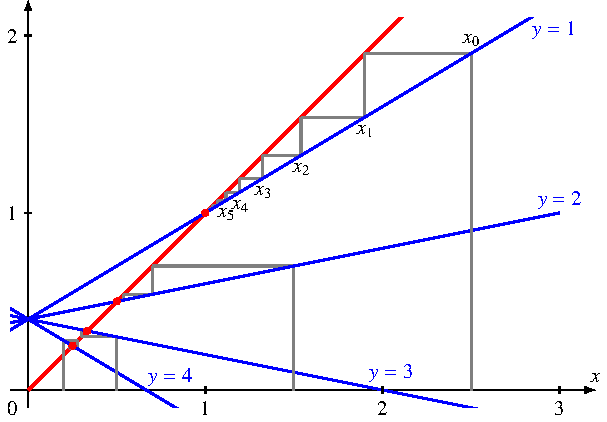
\includegraphics{chapters/1a-frames/images/iteration.pdf}
\caption{Iteration zur Bestimmung des Kehrwertes einer Zahl aus dem
Intervall $[1,5]$ mit der Iterationsformel
$x_{n+1} = f_y(x_n)=x_n + \frac13(1-yx_n)$.
Der Graph von $f_y(x)$ ist eine Gerade durch den Punkt $(0,\frac13)$.
Die Graphen für $f_1$, $f_2$, $f_3$ und $f_4$ sind blau eingezeichnet.
Die Iteration beginnend by einem Startwert $x_0$ führt auf einen 
grau dargestellten Pfad, der sich dem Fixpunkt $y^{-1}$ von $f_y(x)$
nähert.
\label{figure:reziprok}
}
\end{figure}

\begin{beispiel}
Wir verwenden das Verfahren, um den Wert von $1/3$ zu berechnen, also
für $y=3$.
Das Verfahren soll beliebige Werte zwischen $A=2$ und $B=5$ berechnen können.
Mit dem Startwert $x_0=0$ bekommen wir die Werte in
Tabelle~\ref{ginv:iteration:table}.
\begin{table}
\centering
\begin{tabular}{>{$}r<{$}|>{$}l<{$}}
n&x_n\\
\hline
 0&0.000000000000000\\
 1&0.285714285714286\\
 2&0.\underline{3}26530612244898\\
 3&0.\underline{33}2361516034985\\
 4&0.\underline{333}194502290712\\
 5&0.\underline{3333}13500327245\\
 6&0.\underline{33333}0500046749\\
 7&0.\underline{33333}2928578107\\
 8&0.\underline{333333}275511158\\
 9&0.\underline{3333333}25073023\\
10&0.\underline{33333333}2153289\\
11&0.\underline{333333333}164756\\
12&0.\underline{3333333333}09251\\
13&0.\underline{3333333333}29893\\
14&0.\underline{33333333333}2842\\
15&0.\underline{333333333333}263\\
16&0.\underline{3333333333333}23\\
17&0.\underline{33333333333333}2\\
18&0.\underline{333333333333333}\\
\end{tabular}
\caption{Iterative Berechnung von $\frac13$ mit Hilfe der Iterationsformel
von Satz~\ref{satz:reziprok}.
Korrekte Ziffern sind unterstrichen, in jedem Iterationsschritt nimmt
die Anzahl korrekter Ziffern um den gleichen Betrag zu, dies ist
lineare Konvergenz, der Fehler geht wie eine geometrische Folge
gegen $0$.
\label{ginv:iteration:table}
}
\end{table}
In jeder Iteration gewinnt man die gleiche Anzahl korrekter Stellen
(unterstrichen).
Aus dem Beweis von Satz~\ref{satz:reziprok} kann man ablesen,
dass die Konvergenzgeschwindigkeit
\[
\frac{A+B-2y}{A+B}
=
\frac{7-6}{7} = \frac17
\]
ist, man gewinnt also
$\log 7=0.84510$
Stellen in jeder Iteration, in Übereinstimmung mit den obigen numerischen
Resultaten.

Für jeden beliebigen Wert von $y$ im gegebenen Intervall ist die
Konvergenzgeschwindigkeit besser als
$\vartheta=3/7 = 0.42857142\dots$.
Die Anzahl Stellen, die man pro Iteration gewinnt ist daher 
$-\log\vartheta = 0.36798$.
Diese Konvergenzgeschwindigkeit erreicht man an den Enden des Intervalls.
Dazwischen kann man, wie oben gezeigt, deutlich schnellere Konvergenz haben.
\end{beispiel}

%
% Invertierung einer positiv definiten symmetrischen Matrix
%
\subsection{Invertierung einer positiv definiten symmetrischen Matrix $G$
\label{subsection:ginv}}
In diesem Abschnitt ist $G$ eine positiv definite symmetrische Matrix 
mit Eigenwerten im Intervall $[A,B]$.
In Satz~\ref{satz:reziprok} haben wir einen iterativen Algorithmus
gefunden, der jeden Eigenwert von $G$ invertieren kann.


\begin{satz}
\label{satz:ginv}
Ist $G$ eine positiv definite symmetrische Matrix mit Eigenwerten im
Intervall $[A,B]$ und $y\in\mathbb R^n$ dann konvergiert die Folge
\[
x_{n+1} = x_n + \frac{2}{A+B} (y - Gx_n),\qquad x_n = 0
\]
gegen 
$
x=\lim_{n\to\infty} x_n
$
mit $Gx=y$.
\end{satz}

\begin{proof}[Beweis]
Wie im Beweis von Satz~\ref{satz:reziprok} betrachten wir die
Iterationsfunktion
\[
f(x) = x + \frac{2}{A+B}(y-Gx),
\]
wobei $x\in\mathbb R^n$.
Wir müssen zeigen, dass diese Abbildung eine Kontraktion ist, dass
also der Abstand zwischen aufeinanderfolgenden Folgengliedern 
\begin{equation}
\left.
\begin{aligned}
x_{n+1} &= x_n + \frac{2}{A+B}(y-Gx_n)
\\
x_n &= x_{n-1} + \frac{2}{A+B}(y-Gx_{n-1})
\end{aligned}
\right\}
\quad
\Rightarrow
\quad
x_{n+1}- x_{n}
=
x_n-x_{n-1} \frac{2}{A+B}G(x_n-x_{n-1})
\label{inv:iteration:vector}
\end{equation}
in geometrischer Folge abnimmt.
Die rechte Seite von \eqref{inv:iteration:vector}
ist
\begin{equation}
x_n-x_{n-1} \frac{2}{A+B}G(x_n-x_{n-1})
=
\biggl(E-\frac{2}{A+B}G\biggr) (x_n-x_{n-1}).
\label{inv:iteration:vector1}
\end{equation}
Wir müssen die rechte Seite abschätzen.
In einer Eigenbasis ist $G$ eine Diagonalmatrix mit Einträgen zwischen
$A$ und $B$.
Die grosse Klammer auf der rechten Seite von \eqref{inv:iteration:vector1}
ist in dieser Basis die Matrix
\[
E-\frac{2}{A+B}G
=
\begin{pmatrix}
1-\frac{2\lambda_1}{A+B} &            0             &\dots &        0         \\
          0              & 1-\frac{2\lambda_2}{A+B} &\dots &        0         \\
      \vdots             &          \vdots          &\ddots&     \vdots       \\
          0              &            0             &\dots & 1-\frac{2\lambda_n}{A+B}
\end{pmatrix}.
\]
Die Einträge auf der Diagonalen sind
\begin{align}
1-
\frac{2 \lambda_i }{A+B}
&=
\frac{2}{A+B}
\biggl(
\frac{A+B}2 - \lambda_i
\biggr).
\label{inv:iteration:vector2}
\end{align}
Der Wert $(A+B)/2$ ist der Mittelpunkt des Intervalls $[A,B]$, die Eigenwerte
sind also höchstens die halbe Intervallänge $(B-A)/2$ vom Mittelpunkt
entfernt.
Die grosse Klammer auf der rechten Seite von~\eqref{inv:iteration:vector2}
ist daher betragsmässig höchstens $(B-A)/2$.
Nehmen wir den Betrag von~\eqref{inv:iteration:vector2}, erhalten wir
\[
\biggl|
1-
\frac{2 \lambda_i }{A+B}
\biggr|
\le 
\biggl|
\frac2{A+B}
\biggr|
\cdot \frac{B-A}2
=
\frac{B-A}{B+A}=\vartheta.
\]
Aus dem Beweis von Satz~\ref{satz:reziprok} ist bereits bekannt, dass
$0<\vartheta < 1$.

Aus \eqref{inv:iteration:vector} leiten wir jetzt ab, dass
\[
|x_{n+1} - x_n|
\le \vartheta |x_n-x_{n-1}|
\le \dots \le \vartheta^n |x_1-x_0|=\vartheta^n |x_1|.
\]
Die Unterschiede zwischen aufeinanderfolgenden Folgengliedern
nehmen also geometrisch ab.
Aus Lemma~\ref{lemma:konvergenz} folgt daher wie früher, dass
die Folge $(x_n)_{n\in\mathbb N}$ geometrisch gegen den Grenzwert
$x=\lim_{n\to\infty}$
konvergiert.

Wir müssen jetzt nur noch zeigen, dass $x$ tatsächlich das Bild von $y$
unter $G^{-1}$ ist.
Gehen wir in der Iterationsfolge zum Grenzwert über, folgt
\[
x_{n+1} = x_n + \frac{2}{A+B}(y-Gx_n)
\qquad\rightarrow\qquad
x = x + \frac{2}{A+B}(y-Gx).
\]
Die $x$ auf beiden Seiten des Gleichheitszeichens rechts
heben sich weg.
Den Faktor $2/(A+B)$ kann man wegkürzen, da er nie verschwindet.
Es bleibt
\[
0
=
y-Gx
\qquad
\Rightarrow
\qquad
y=Gx,
\]
$x$ ist also der gesucht Urbildvektor.
\end{proof}

\begin{beispiel}
Wir verwenden die Iteration des Satzes \ref{satz:ginv} zur Berechnung
der Inversen der Matrix
\[
G=\begin{pmatrix}2&1&0\\1&2&1\\0&1&2\end{pmatrix}.
\]
Zunächst benötigen wir die Framekonstanten $A$ und $B$.
Diese müssen nicht exakt bekannt sein, es muss nur sichergestellt sein,
dass alle Eigenwerte $\lambda$ von $G$ im Intervall $[A,B]$ liegen.
Das charakteristische Polynom von $G$ ist
\[
\chi_{G}(\lambda)
=
\det(G-\lambda E)
=
\left|
\begin{matrix}
2-\lambda&1&0\\1&2-\lambda&1\\0&1&2-\lambda
\end{matrix}
\right|
=
(2-\lambda)^3-2(2-\lambda).
\]
Auf der rechten Seite lässt sich ein Faktor $(2-\lambda)$ ausklammern.
So erhält man
\begin{align*}
\chi_{G}(\lambda)
&=
(2-\lambda)\bigl((2-\lambda)^2-2\bigr)
=
(2-\lambda)
(\lambda^2 -4\lambda+2).
\end{align*}
Der quadratische Term auf der rechten Seite hat die Nullstellen
\[
\lambda_{\pm} = 2 \pm \sqrt{4-2} = 2 \pm\sqrt{2},
\]
damit kann man das charakteristische Polynom weiter faktorisieren
in
\[
\chi_{G}(\lambda)
=
(2-\lambda)
(\lambda -2-\sqrt{2})(\lambda -2+\sqrt{2}).
\]
Die Eigenwerte von $G$ sind daher
\[
2-\sqrt{2},\quad
2,\quad
2+\sqrt{2}.
\]
Die exakten Werte für $A$ und $B$ sind daher
\[
A=2-\sqrt{2}
\qquad\text{und}\qquad
B=2+\sqrt{2}.
\]
Der zugehörige Wert von $\vartheta$, der die Konvergenzgeschwindigkeit
definiert, ist $\vartheta = (A-B)/(A+B)=2\sqrt{2}/4=\sqrt{2}/2=0.707$.
Man leitet daraus ab, dass für jede Stelle Genauigkeit 6 Iterationsschritte
benötigt.
Für ein auf 5 Stellen exaktes Resultat muss man daher mit mindestens 30
Iterationsschritten rechnen.

Die Iterationsformel ist in beiden Fällen
\[
x_{n+1} = x_n + \frac12(y-Gx_n)
\]
mit Startwert $x_0=0$.
Für den ersten Standardbasisvektor $y=e_2$ findet man die Iterationsfolge
\begin{align*}
x_1 &=
\begin{pmatrix}
   0.0\\
   0.5\\
   0.0
\end{pmatrix},
&
x_2 &=
\begin{pmatrix}
  -0.25\\
 \phantom{-}  0.50\\
  -0.25
\end{pmatrix},
&
x_3 &=
\begin{pmatrix}
  -0.20\\
   \phantom{-}0.70\\
  -0.20
\end{pmatrix},
&
x_4 &=
\begin{pmatrix}
  -0.375\\
   \phantom{-}0.750\\
  -0.375
\end{pmatrix},
&
x_5 &=
\begin{pmatrix}
  -0.375\\
   \phantom{-}0.875\\
  -0.375
\end{pmatrix},
\\
x_6 &=
\begin{pmatrix}
  -0.4375\\
   \phantom{-}0.8750\\
  -0.4375
\end{pmatrix},
&
x_7 &=
\begin{pmatrix}
  -0.4375\\
   \phantom{-}0.9375\\
  -0.4375
\end{pmatrix},
&
x_8 &=
\begin{pmatrix}
  -0.46875\\
   \phantom{-}0.93750\\
  -0.46875
\end{pmatrix},
&
x_9 &=
\begin{pmatrix}
  -0.46875\\
   \phantom{-}0.96875\\
  -0.46875
\end{pmatrix},
&
x_{10} &=
\begin{pmatrix}
  -0.48438\\
   \phantom{-}0.96875\\
  -0.48438
\end{pmatrix},
\dots
\end{align*}
Die relative langsame Konvergenz kann gut verfolgt werden.
Der Grenzwert ist
\[
x_{\infty} = \lim_{n\to\infty}x_n = \begin{pmatrix}
-0.5\\\phantom{-}1.0\\-0.5
\end{pmatrix}.
\]
Führt man die Iteration für die anderen Standardbasisvektoren durch,
findet man als Grenzmatrix
\[
H=\frac14\begin{pmatrix}
 3&-2& 1\\
-2& 4&-2\\
 1&-2& 3
\end{pmatrix}
\]
und man kann leicht nachprüfen, dass $GH=E$.
\end{beispiel}

Im Beispiel wurde jeder Standardbasisvektor einzeln invertiert.
Dabei wurde immer die gleiche Operation
\[
x = x - \frac{2}{A+B}(y - Gx)
\]
angewendet.
Schreibt man alle Standardbasisvektoren in eine Matrix erhält man 
die Einheitsmatrix $E$. Aus den zugehörigen Vektoren $x_n$
wird die Matrix $H_n$, dann lässt sich die Operation auch als
Matrizenoperation
\[
H \to H - \frac{2}{A+B}(E - GH)
\]
schreiben.
Da jede einzeln Spalte mit der gleichen, durch $\vartheta = (B-A)/(B+A)$
definierten Geschwindigkeit konvergiert, kann der Satz auch als
Iterationsverfahren für die inverse Matrix formuliert werden.

\begin{satz}
Ist $G$ eine symmetrische Matrix derart, dass ihre Eigenwerte im
Intervall $[A,B]$ mit $0<A\le B$ enthalten sind, dann konvergiert
die Matrixfolge
\[
H_{n+1}
=
H_n
+
\frac{2}{A+B}
(
E-
GH_n
)
,
\qquad
H_0=0
\]
linear gegen den Matrix $H$ mit der Eigenschaft $GH=E$.
Der Fehler nimmt in jeder Iteration mindestens um den Faktor
$\vartheta=(B-A)/(A+B)$ ab.
\end{satz}









%
% plancherel.tex
%
% (c) 2019 Prof Dr Andreas Müller, Hochschule Rapperswil
%
\section{Plancherel-Formel%
\label{section:cwt:plancherel}}
\rhead{Plancherel-Formel}
Die Plancherel-Formel der Fourier-Theorie besagt, dass die
Fourier-Transformation eine Isometrie ist.
Das Skalarprodukt zweier Funktionen und das Skalarprodukt der
Fourier-Transformierten ist dasselbe.
Daraus folgt unmittelbar, dass die Transformation stetig und
umkehrbar ist.
Es ist daher erstrebenswert, wenn eine ähnliche Formel auch
auch für die stetige Wavelet-Transformation gilt.

\subsection{Das Skalarprodukt auf $H$}
Der Definnitionsbereich $H=\mathbb R^* \times \mathbb R$ der
Wavelet-Transformierten kan auf verschiedene Arten mit einer Integration
ausgestattet werden.
Wir versuchen das ``richtige'' Mass zu erraten, im
Abschnitt~\ref{subsection:haar-mass} werden wir eine abstrakte Begründung
geben.

Die Variable $b$ verhält sich genau wie die Variable $t$ bei Integration
einer Funktion von $t$.
Funktionen werden durch den Parameter $b$ verschoben, dabei darf sich
das Integral nicht ändern.
Das ist genau die Eigenschaft, mit deren Hilfe das Lebesgue-Mass
definiert wurde.

Die Variable $a$ funktioniert dagegen als Skalierungsparameter.
Grössere Werte von $a$ ziehen den Träger des Integranden um den Faktor $a$ 
in die Länge.

\begin{definition}
\label{cwt:definition:plancherel}
Das Mass auf $H$ ist definiert duch das Integral
\[
\int_H F(a,b)\,db \,\frac{da}{a^2}
\]
und das Skalaprodukt von Funktionen auf $H$ ist
\[
\langle F,G\rangle_H
=
\int_{H} F(a,b)\overline{G(a,b)}\,db \,\frac{da}{a^2}.
\]
\end{definition}

Dieses Mass ist im folgenden Sinn das richtige Mass.
Wenden wir auf die Argumente einer Funktion auf $H$ die Transformation
\[
(a,b) \mapsto (\alpha a, \beta + \alpha b)
\]
an, ändert sich das Integral wie folgt:
\begin{align*}
\int_H F(\alpha a,\beta + \alpha b)\,d(\beta + \alpha b)\,\alpha\frac{da}{|\alpha a|^2}
&=
\int_H F(\alpha a,\beta + \alpha b) \alpha\,db \ \frac{da}{|a|^2},
\end{align*}
die Transformation der Funktion ändert also das Integral nicht.
Die Wahl des Integrals ist so, dass die Skalierung und Translation
das Integral nicht ändert.

\subsection{Die Abhängigkeit von $b$}
Die partielle Funktion $b\mapsto \mathcal{W}f(a,b)$ ist etwas einfacher
zu verstehen, wir versuchen sie daher zunächst für konstantes $a$
anders auszudrücken.
Da die Wavelet-Transformierte ein Skalarprodukt in $L^2(\mathbb R)$
ist, können wir die Plancherel-Formel für die Fouriertransformation
verwenden und erhalten.
\[
\mathcal{W}f (a,b)
=
\langle f,\psi_{a,b} \rangle
=
\langle \hat{f}, \hat{\psi}_{a,b}\rangle.
\]
Die Fouriertransformierte von $\psi_{a,b}$ ist aber bereits bekannt,
sie ist
\[
\hat{\psi}_{a,b}(\omega)
=
e^{-i\omega b} \hat{\psi}_a(\omega)
=
\sqrt{|a|}e^{-i\omega b} \hat{\psi}(a\omega).
\]
Damit kann jetzt die Wavelet-Transformierte als Skalarprodukt im
Frequenzraum geschrieben werden:
\begin{align*}
\mathcal{W}f (a,b)
&=
\int_{-\infty}^\infty 
\hat{f}(\omega)
\sqrt{|a|}e^{i\omega b} \overline{\hat{\psi}(a\omega)}
\,d\omega
=
\int_{-\infty}^\infty
\bigl(
\sqrt{|a|}
\hat{f}(\omega)
\overline{\hat{\psi}(a\omega)}
\bigr)
e^{i\omega b}
\,d\omega
\\
&=
\frac1{\sqrt{2\pi}}
\int_{-\infty}^\infty
\underbrace{
\sqrt{2\pi}
\sqrt{|a|}
\hat{f}(\omega)
\overline{\hat{\psi}(a\omega)}}_{\displaystyle F_a(\omega)}
e^{i\omega b}
\,d\omega
\end{align*}
Daraus kann man ablesen, dass $F_a(\omega)$ die Fourier-Umkehrtransformierte
der Funktion $b\mapsto \mathcal{W}f(a,b)$ ist.
Bezeichnen wir die Fourier-Umkehrtransformierte mit dem umgekehrten
Dach über dem Funktionsbuchstaben,
dann folgt
\begin{equation}
\check{F}_a(b) = \mathcal{W}f(a, b)
\label{cwt:checkF}
\end{equation}

\subsection{Die Plancherel-Formel}
Ziel dieses Abschnitts ist, in Satz~\ref{satz:wplancherel} die
Plancherel-Formel für die Wavelet-Transformation zu beweisen.
Wir wollen diesen Beweis auf die Plancherel-Formel für die 
Fourier-Transformation stützen, die bereits die Formel~\eqref{cwt:checkF}
für die $b$-Abhängigkeit geliefert hat.
Wir werden natürlich wieder die Funktion $F_a(\omega)$ benötigen.
Da die Plancherel-Formel das Skalarprodukt zweier Funktionen berechnet,
werden wir eine zweite Funktion $g$ bezeichnen, die zugehörige, analog
zu $F_a(\omega)$ gebildete Funktion wird mit $G_a(\omega)$ bezeichnet,
es ist
\[
G_a(\omega)
=
\sqrt{2\pi}\sqrt{|a|}
\hat{g}(\omega)
\overline{\hat{\psi}(a\omega)}.
\]
Damit sind wir jetzt in der Lage, die Plancherel-Formel zu beweisen:

\begin{satz}
\label{satz:wplancherel}
Sei $\psi$ ein Wavelet mit der Konstanten $C_{\psi}$, wie sie in
der Zulässigkeitsbedingung auftritt.
Dann gilt
\begin{equation}
\langle \mathcal{W}f,\mathcal{W}g\rangle
=
C_{\psi}\langle f,g\rangle
\end{equation}
für beliebige Funktionen $f,g\in L^2$.
\end{satz}

\begin{proof}[Beweis]
Wir verwenden 
\begin{align}
\langle \mathcal{W}f, \mathcal{W}g\rangle_H
&=
\int_{\mathbb R^*} \int_{-\infty}^\infty
\mathcal{W}f (a,b)
\overline{\mathcal{W}g (a,b)} \,db \,\frac{da}{|a|^2}
\notag
\\
&=
\int_{\mathbb R^*} \int_{-\infty}^\infty
\hat{F}_a(b) \overline{\hat{G}_a(b)}\,db\,\frac{da}{|a|^2}
\notag
\\
&=
\int_{\mathbb R^*} 
\langle
\check{F}_a,\check{G}_a
\rangle
\,\frac{da}{|a|^2}
\notag
\\
&=
\int_{\mathbb R^*} \langle F_a, G_a\rangle \,\frac{da}{|a|^2}
\notag
\\
&=
\int_{\mathbb R^*}
\int_{-\infty}^\infty
2\pi |a|\hat{f}(\omega) \overline{\hat{g}(\omega)} |\hat{\psi}(a\omega)|^2
\,d\omega
\,\frac{da}{|a|^2}
\notag
\\
&=
\int_{-\infty}^\infty
\hat{f}(\omega) \overline{\hat{g}(\omega)}
\underbrace{
2\pi
\int_{\mathbb R^*}
|\hat{\psi}(a\omega)|^2
\,\frac{da}{|a|}}_{\displaystyle=C_\psi}
\,d\omega.
\label{cwtplancherel:p1}
\end{align}
Das Produkt $\hat{f}(\omega)\overline{\hat{g}(\omega)}$ deutet darauf hin,
dass dies fast schon ein Skalarprodukt ist.
Es wird tatsächlich das Skalarprodukt, wenn das innere Integral konstant ist.
Wir betrachten dieses separat und setzen $a\omega = s$, was
\begin{align*}
\int_{\mathbb R^*} |\hat{\psi}(a\omega)|^2 \,\frac{da}{|a|}
&=
\int_{\mathbb R^*} |\hat{\psi}(s)|^2 \,\frac{ds/\omega}{|s/\omega|}
=
\int_{\mathbb R^*} |\hat{\psi}(s)|^2 \,\frac{ds}{|s|}
=
\frac{C_{\psi}}{2\pi}
\end{align*}
ergibt.
Eingesetzt in \eqref{cwtplancherel:p1} finden wir
\begin{align*}
\langle \mathcal{W}f, \mathcal{W}g\rangle_H
&=
C_{\psi}
\int_{-\infty}^\infty \hat{f}(\omega)\overline{\hat{g}(\omega)}\,d\omega
=
C_{\psi}
\langle \hat{f},\hat{g}\rangle
=
C_{\psi}
\langle f,g\rangle.
\end{align*}
Damit ist die Plancherel-Formel bewiesen.
\end{proof}

Mit dem Satz~\ref{satz:wplancherel} wird jetzt klar, warum die
Zulässigkeitsbedingung so wichtig ist.
Die Zulässigkeitsbedingung ist genau das was wir brauchen um zu schliessen,
dass die stetige Wavelet-Transformation stetig ist.
Aus dem Satz folgt, dass
\[
\| \mathcal{W}f \|_H = \sqrt{C_{\psi}}\|f\|.
\]
Es ist also nicht möglich, dass eine Funktion $f\ne 0$ eine verschwindende
Wavelet-Transformation hat.
Anders ausgedrückt: verschiedene Funktionen lassen sich immer auch anhand
ihrer Wavelet-Transformation unterscheiden.

\subsection{Das Haar-Mass auf $\mathbb R^* \ltimes \mathbb R$
\label{subsection:haar-mass}}
Das Lebesgue-Mass auf $\mathbb R$ zeichnet sich dadurch aus, dass
die Translation einer Funktion ein Integral nicht ändert:
\[
\int_{\mathbb R} T_bf(t)\,dt
=
\int_{\mathbb R} f(t-b)\,dt
=
\int_{\mathbb R} f(t)\,dt.
\]
Diese Eigenschaft kann man auch in anderen Definitionsbereichen antreffen.
Zum Beispiel ändert sich das Integral
\[
\int_0^\infty f(t)\,\frac{dt}{t}
\]
auch nicht, wenn die Funktio $f$ durch $\tilde{D}_af$ ersetzt wird
für $a>0$.
Die Substition $\tau = t/a$ im Integral
\begin{align*}
\int_0^\infty \tilde{D}_af(t)\,\frac{dt}{t}
&=
\int_0^\infty f(t/a)\,\frac{dt}{t}
=
\int_0^\infty f(\tau) \frac{a d\tau}{a\tau}
=
\int_0^\infty f(\tau) \frac{d\tau}{\tau}
\end{align*}
zeigt dies.
So wie $\mathbb R$ abgeschlossen ist bezüglich der Addition ist die Menge
$\mathbb R^+=\{x\in\mathbb R\;|\; x > 0\}$ abgeschlossen unter Multiplikation.

Diese Beboachtung lässt sich weitgehend verallgemeinern.
Eine {\em Gruppe} ist eine Menge mit einer assoziativen Operation, einem
bezüglich der Operation neutralen Element und so, dass jedes Element
invertierbar ist.
Die Menge $\mathbb R$ ist eine Gruppe bezüglich der Addition mit dem neutralem
Element $0$ und dem inversen Element $-x$ zu jedem $x\in\mathbb R$.
Für die Menge $\mathbb R^+$ mit der Multipliation als Operation ist
$1$ das neutrale Element und das inverse Element von $x\in\mathbb R^+$
ist $x^{-}$.
Die beiden Beispiel zeigen, dass es unter gewissen Voraussetzungen
möglich ist, für Funktionen auf einer Gruppe $G$ ein Integral zu definieren,
welches unverändert bleibt, wenn man die Funktion $f:G\to \mathbb C$ 
durch die Funktion $(g\cdot f)(x) = f(g\cdot x)$ ersetzt, also
\[
\int_G (g\cdot f)(x)\,d\mu(x)
=
\int_G f(x)\,d\mu(x).
\]
Die Existenz eines solchen Masses ist nicht trivial und wurde
von Alfréd Haar 1933 bewiesen. 
\index{Alfréd Haar}
\index{Haar, Alfréd}
Es wird heutzutage {\em Haarsches Mass} genannt.
\index{Haar Mass}

Die Menge $H=\mathbb R^*\times \mathbb R$ ist eine Gruppe mit der
Gruppenoperation
\[
(a_1,b_1)\cdot (a_2,b_2) = (a_1a_2,a_1b_2+b_1),
\]
dem neutralen Element $(1,0)$ und dem inversen Element
\[
(a,b)^{-1} = (a^{-1}, -a^{-1}b)
\qquad\text{denn}\qquad
\left\{
\begin{aligned}
(a,b)\cdot (a^{-1},-a^{-1}b)
&=
(aa^{-1},b-aa^{-1}b)=(1,0)
\\
(a^{-1},-a^{-1}b)\cdot (a,b)
&=
(a^{-1}a,-a^{-1}b-a^{-1}b)=(1,0).
\end{aligned}
\right.
\]
Die Gruppe $H$ wird auch $H=\mathbb R^*\times \mathbb R$ geschrieben
und heisst das semidirekte Produkt der Gruppen $\mathbb R^*$ mit der
Multiplikation als Gruppenoperation und $\mathbb R$ mit der Addition
als Gruppenoperation.
Nach Haar müsste es also auch ein Haarsches Mass auf $H$ geben.

$H$ enthält zwei Gruppen, für die wir das Haarsche Mass schon kennen.
Für $\mathbb R$ ist es das gewöhnliche Lebesgue-Integral, für $\mathbb R^*$
ist es ein Integral mit einem Faktor $1/x$.
Man kann daher vermuten, dass das Haar-Integral von der Form
\[
\int_H f(a,b) \,\frac{da}{m(a)}\,db
\]
sein muss.

Wenden wir die Operation des Gruppen-Elements $(\alpha,\beta)\in H$
auf die Funktion $f$ an und verwenden die Substitution
$\tilde{a}=\alpha a$ und $\tilde{b}=\alpha b$
\begin{align*}
\int_H f(\alpha a,\beta-\alpha b) \,\frac{da}{m(a)}\,db
&=
\int_H f(\tilde{a}, \beta - \tilde b) \,
d\tilde{b}/\alpha\,\frac{d\tilde{a}/\alpha}{m(a)}
\\
&=
\int_H f(\tilde{a}, \beta - \tilde b) \,
d\tilde{b}\,\frac{d\tilde{a}}{\alpha^2m(a)}
\\
&=
\int_H f(\tilde{a}, \beta) \,
d\tilde{b}\,\frac{d\tilde{a}}{\alpha^2m(a)}.
\end{align*}
Das Integral ändert sich genau dann nicht, wenn
\[
\alpha^2 m(a)
=
m(\tilde{a})
=
m(\alpha a)
\qquad\Rightarrow\qquad
m(a) = a^2.
\]
Dies ist genau das in der Definition~\ref{cwt:definition:plancherel}
des Skalarproduktes für die stetige Wavelettransformation verwendete
Integral.







\section*{Übungsaufgaben}
\rhead{Übungsaufgaben}
\uebungsaufgabe{01001}
\uebungsaufgabe{01002}
\uebungsaufgabe{01003}
\uebungsaufgabe{01004}
\uebungsaufgabe{01005}






